\chapter{Transfer learning from ImageNet}

%%%%%%%%% ABSTRACT
% \begin{abstract}
% In this paper, we study deep transfer learning as a way of overcoming object recognition challenges encountered in the field of digital pathology. Through several experiments, we investigate various uses of pre-trained neural network architectures and different combination schemes with random forests for feature selection. Our experiments on eight classification datasets show that densely connected and residual networks consistently yield best performances across strategies. It also appears that network fine-tuning and using inner layers features are the best performing strategies, with the former yielding slightly superior results. 
% \end{abstract}



%-------------------------------------------------------------------------------------------------------------------
%-------------------------------------------------------------------------------------------------------------------
%%%%%%%%% BODY TEXT
\section{Introduction}

In pathology, tissues were traditionally examined under an optical microscope after being sectioned, stained and mounted on a glass slide. During the last years, progress in scanning technologies made possible the high-throughput digitization of glass slides at high resolution. Digital pathology holds promise for biomedical research and clinical routine but raises great challenges for computer vision research \parencite{automated-histology-signal-proc-2014}. 
First and foremost, a laboratory can produce and scan large amounts of slides per day, each of them being a multi-gigapixel image. Moreover, those slides can contain many different kinds of tissues with different staining techniques. Their quantity, variability and size therefore require efficient and versatile computer vision methods. The second challenge is the scarcity of annotated data. Indeed, annotations of digitized slides require expertise and are therefore expensive and tedious to obtain.

In parallel, deep learning has recently had an impressive impact over the computer vision field starting with work of Krizhevsky \etal \parencite{krizhevsky2012imagenet}, which improved previous natural image recognition performances by a large margin. More recently, researchers have been working at applying those new techniques to biomedical imaging \parencite{greenspan2016guest,litjens2017survey}. While current results are promising, improvements were not as impressive as they had been for traditional computer vision tasks (recognition of natural scenes or objects such as ImageNet \parencite{deng2009imagenet}, face recognition...) which can likely be attributed to the lack of annotated data.

Interestingly, works such as \parencite{donahue2014decaf,yosinski2014transferable,sermanet2013overfeat} have shown that convolutional neural networks can be used efficiently for transfer learning, \ie a network can be trained on a source task and then be reused on a target task. This technique is particularly handy when the data for the target task is scarce and one has a large dataset that can be used for training as source task. Therefore, it is not surprising that deep transfer learning has been studied by the biomedical imaging community to overcome the data scarcity problem. In their review \parencite{litjens2017survey}, Litjens \etal identify two transfer learning strategies for image classification: using off-the-shelf features extracted from pre-trained networks or fine-tuning these latter networks for the task at hand. The first strategy uses features learned from the source task without re-training the network and use them to train a third-party classifier. Extracting such features is usually fast (with ad-hoc computing resources, \ie graphical processing units) and this approach requires only to tune the hyper-parameters of the final classifier, which can usually be done efficiently through cross-validation. Those properties make off-the-shelf features particularly appealing for biomedical imaging given the aforementioned challenges. The second strategy consists in using a network initialized with pre-trained weights and partially re-training it on the target task. This approach is more computationally demanding than using off-the-shelf features and involves dealing with more hyper-parameters. In terms of performance, as stated in \parencite{litjens2017survey}, both strategies have not been compared thoroughly yet in biomedical imaging and there is no consensus about whether one is better than the other.

In this work, we study thoroughly and compare several strategies that involve off-the-shelf features and network fine-tuning. We carry out several experiments over eight object classification datasets in digital histology and cytology. Different combinations of state-of-the-art networks and feature selection techniques using random forests are proposed in order to answer questions of very high pratical relevance: which network provides best-performing features? How should those features be extracted and then exploited to get the best performance? Is fine-tuning better than using off-the-shelf features? More generally, our empirical study will also contribute to confirm the interest of deep transfer learning for tackling the recurrent data scarcity problem in biomedical imaging.





%-------------------------------------------------------------------------------------------------------------------
%-------------------------------------------------------------------------------------------------------------------
\section{Related work}

Transfer learning has been studied for a long time \parencite{pan2010survey}, but its applicability in deep learning has only been discovered recently. Decaf \parencite{donahue2014decaf} and Overfeat \parencite{razavian2014cnn,sermanet2013overfeat} are the first published off-the-shelf feature extractor networks. The former is based on AlexNet \parencite{krizhevsky2012imagenet}, the latter is a custom architecture. Both were pre-trained on ImageNet and provide generic features for computer vision tasks. Those features can then used by other methods such as SVM \parencite{fan2008liblinear} or random forests \parencite{breiman2001random} for final classification. Following those advances, works such as \parencite{yosinski2014transferable,zeiler2014visualizing} shed more light on the transfer learning process by empirically analyzing the extracted features for various tasks. One interesting conclusion of these works is that shallow features seem to be generic whereas deep ones are more specific to the source task.

Some of the first applications of deep transfer learning in biomedical imaging were reported in \parencite{bar2015chest,ciompi2015automatic,van2015off} for pulmonary nodule detection in chest x-rays and CT-scans using Decaf and OverFeat. While those works have revealed the potential of deep transfer learning in that field, the performances were not significantly better than those of previous methods. More recently, fine-tuning has been also investigated and compared with networks trained from scratch and classifiers trained on off-the-shelf features on a wide variety of biomedical imaging tasks \parencite{antony2016quantifying,esteva2017dermatologist,gulshan2016development, ravishankar2016understanding,shin2016deep,tajbakhsh2016convolutional}. More specifically, digital pathology and microscopy are not outdone with works on tissue texture \parencite{kieffer2017convolutional}, cell nuclei \parencite{bayramoglu2016transfer} and breast cancer \parencite{han2017breast} classification from histopathology images or analysis of high-content microscopy data \parencite{kraus2017automated}. Most works have used networks pre-trained on the ImageNet image classification dataset. Others, like \parencite{kraus2017automated}, have used a custom network architecture pre-trained on a medical dataset as source task. 

While it is clear that training from scratch very deep networks is not viable in most case due to data scarcity \parencite{bayramoglu2016transfer,tajbakhsh2016convolutional}, there is currently no consensus and best practice about how transfer learning should be applied to digital pathology and microscopy. Some recent publications in the biomedical field have shown that fine-tuning outperforms off-the-shelf features \parencite{antony2016quantifying,kieffer2017convolutional,ravishankar2016understanding,shin2016deep}. However, as noted in \parencite{litjens2017survey}, experiments in these papers are often carried out on a single dataset, which does not allow to draw general conclusions. Moreover, those experiments do not use current state-of-the-art networks. A short review of the networks used in biomedical imaging is given in Supplementary Table 1 and shows that the more recent and efficient residual and densely connected networks have been underused or not used at all, in particular in digital pathology and microscopy.

%most studies have focused on AlexNet \parencite{krizhevsky2012imagenet}, VGG16 \parencite{simonyan2014very}, GoogLeNet \parencite{szegedy2015going} and InceptionV3 \parencite{szegedy2016rethinking} architectures while






%-------------------------------------------------------------------------------------------------------------------
%-------------------------------------------------------------------------------------------------------------------
\section{Datasets}
\label{sec:comp:datasets}


\begin{table*}
    \center 
    \begin{tabular}{|c|c|c||cc|cc|cc||cc|}
        \hline
        \multirow{2}{*}{Dataset} & \multirow{2}{*}{Domain} & \multirow{2}{*}{Cls} & \multicolumn{2}{c|}{Train} & \multicolumn{2}{c|}{Validation} & \multicolumn{2}{c||}{Test} & \multicolumn{2}{c|}{Total} \\
        \cline{4-11}
        & & & Images & Slides & Images & Slides & Images & Slides & Images & Slides \\
        \hline
        Necrosis (N) & Histo & 2 & 695 & 9 & 96 & 1 & 91 & 3 & 882 & 13 \\ % ulg_lbtd2_chimio_necrose
        ProliferativePattern (P) & Cyto & 2 & 1179 & 19 & 167 & 4 & 511 & 13 & 1857 & 36 \\ % patterns_no_aug
        CellInclusion (C) & Cyto & 2 & 1644 & 21 & 173 & 2 & 1821 & 22 & 3638 & 45 \\ % cells_no_aug
        MouseLba  (M) & Cyto & 8 & 1722 & 9 & 716 & 4 & 1846 & 7 & 4284 & 20 \\ % ulg_lbtd_lba
        HumanLba (H) & Cyto & 9 & 4051 & 50 & 346 & 5 & 1023 & 9 & 5420 & 64 \\ % ulb_anapath_lba
        Lung (L) & Histo & 10 & 4881 & 669 & 562 & 73 & 888 & 140 & 6331 & 882 \\ % ulg_lbtd_tissus
        Breast (B) & Histo & 2 & 14055 & 22 & 4206 & 8 & 4771 & 4 & 23032 & 34 \\ % ulg_breast
        Glomeruli (G) \parencite{maree2016approach} & Histo & 2  & 12157 & 91 & 2448 & 12 & 14608 & 102 & 29213 & 205 \\ % glomeruli_no_aug
        \hline
    \end{tabular}
    \caption{Sizes and splits of the datasets.}
    \label{tab:comp:dataset_information}
\end{table*}

\begin{figure*}
	\center
    \subfloat[Necrosis]{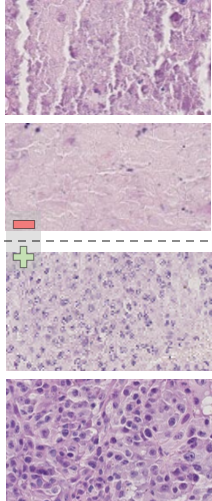
\includegraphics[scale=0.55]{comp/illus_necrose.png}}
    \subfloat[ProliferativePattern]{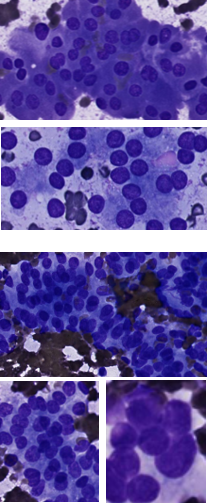
\includegraphics[scale=0.55]{comp/illus_patterns.png}}
    \subfloat[CellInclusion]{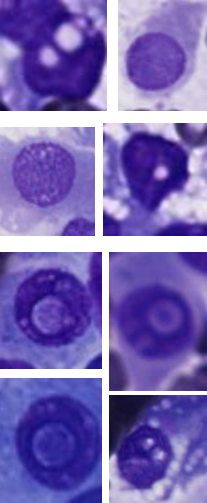
\includegraphics[scale=0.55]{comp/illus_cells.png}}
    \subfloat[Breast]{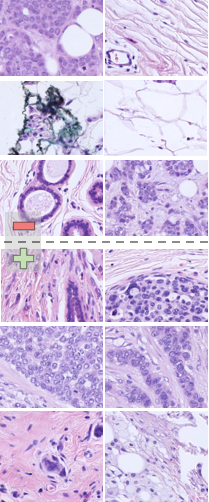
\includegraphics[scale=0.55]{comp/illus_breast.png}}
    \subfloat[Glomeruli]{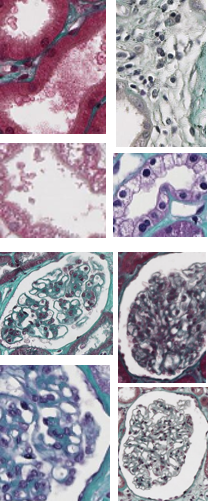
\includegraphics[scale=0.55]{comp/illus_glomeruli.png}}
    \subfloat[MouseLba]{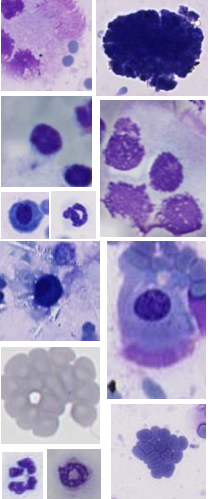
\includegraphics[scale=0.55]{comp/illus_lbtd_lba.png}}
    \subfloat[HumanLba]{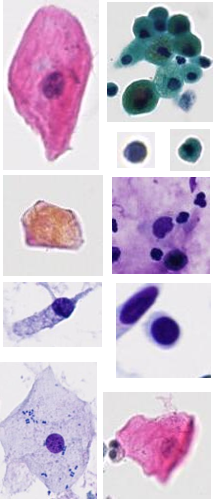
\includegraphics[scale=0.55]{comp/illus_anapath.png}}
    \subfloat[Lung]{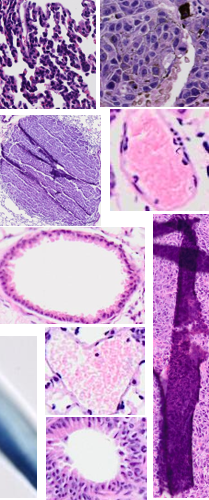
\includegraphics[scale=0.55]{comp/illus_tissus.png}}
	\caption{Overview of our eight classification datasets (the display size does not reflect actual image size). For binary classification datasets, negative and positive samples were respectively placed at the top and bottom of the figures.}
	\label{fig:comp:dataset_samples}
\end{figure*}
 

Our experimental study uses datasets collected over the years by biomedical researchers and pathologists using the Cytomine \parencite{maree2016collaborative} web application. Using this platform, eight image classification datasets were collected which are summarized in Table \ref{tab:comp:dataset_information}. These contain tissues and cells from human or animal organs (thyroid, kidney, breast, lung, \ldots).

For all datasets except Breast, each sample image is the crop of an annotated object extracted from a whole-slide image. The Breast dataset is composed of patches for which the label encodes the type of tissue in which the central pixel is located. Selected image samples for each dataset are shown in Figure \ref{fig:comp:dataset_samples}. 




%-------------------------------------------------------------------------------------------------------------------
%-------------------------------------------------------------------------------------------------------------------
\section{Methods}

%{\color{green} PG: je pense que la structure pourrait \^etre am\'elior\'ee. L'info est un peu bizarrement r\'epartie dans les diff\'erentes sous-sections.}

\label{sec:comp:methods}

%\subsection{Pre-trained networks}




%\subsection{General framework}
%\label{ssec:comp:meth_general_framework}

 
\subsection{Deep networks}
We follow the feature extraction and classification process presented in Figure \ref{fig:comp:diag_feat_extract}, which starts from a deep convolutional neural network $\mathcal{N}$ pre-trained on a source task $S$. In particular, we use ImageNet as the source dataset $S$ and, for each network, the pre-trained weights were retrieved from Keras \parencite{chollet2015keras}. For $\mathcal{N}$, we evaluate several architectures that have been or are state of the art on the ImageNet classification dataset \parencite{deng2009imagenet} or that present interesting trade-off between computational requirements and performances: VGG16, VGG19 \parencite{simonyan2014very}, InceptionV3 \parencite{szegedy2016rethinking}, ResNet50 \parencite{he2016deep}, InceptionResNetV2 \parencite{szegedy2017inception}, DenseNet201 \parencite{huang2017densely}, and MobileNet \parencite{howard2017mobilenets}. In the sequel, those networks will be respectively referred to as VGG16, VGG19, IncV3, ResNet, IncResV2, DenseNet, and Mobile. These networks can be used off-the-shelf or fine-tuned, as explained below.

\subsection{Off-the-shelf feature extraction}

 \begin{figure*}
   \center
   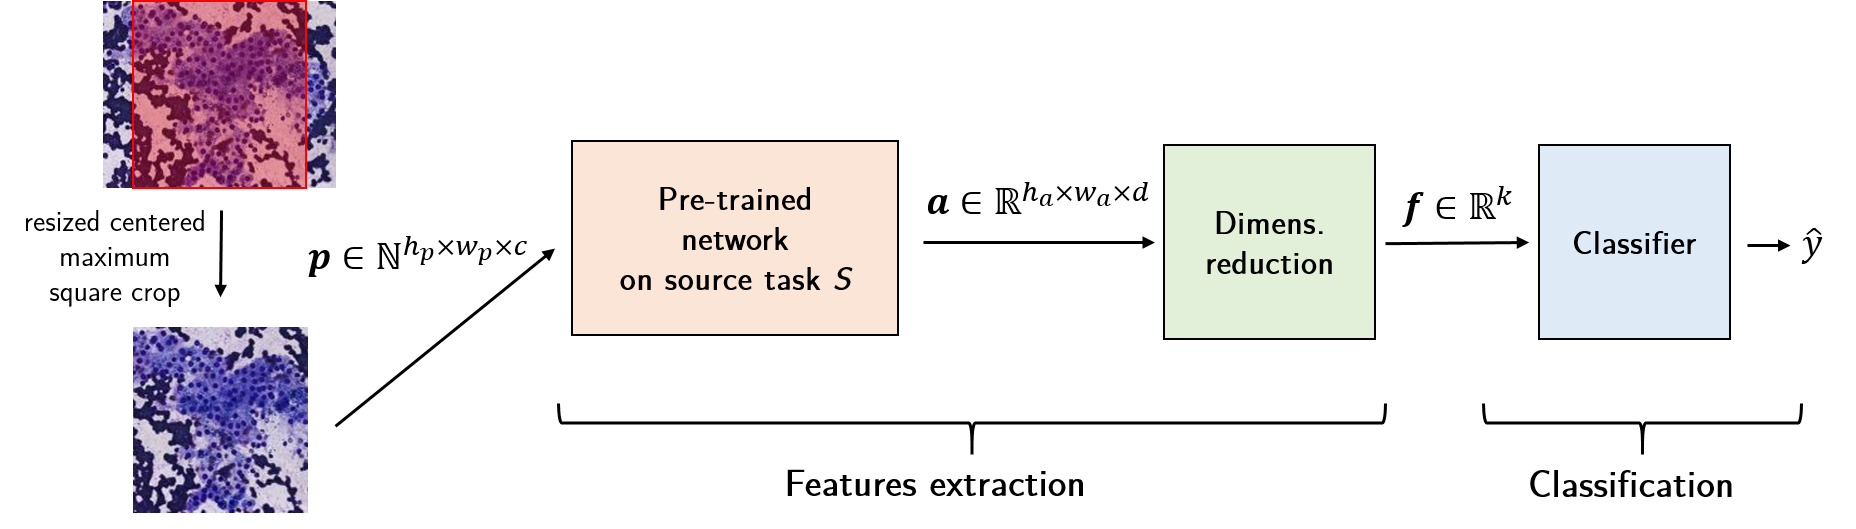
\includegraphics[scale=0.50]{comp/offtheshelf_schema.png}
     \caption{Feature extraction from pre-trained convolutional neural networks}
     \label{fig:comp:diag_feat_extract}
 \end{figure*}


Images are first resized to match the input dimension of the network. Respectively denoting by $h_{\mathcal{I}} \times w_{\mathcal{I}} \times c$ the height, width, and number of channels of the input image ${\cal I}$, we extract a square patch $\mathbf{p}$ of (maximum) height and width $\min(h_{\mathcal{I}}, w_{\mathcal{I}})$ in the center of the image, which is then resized to the network input size $h_p\times w_p\times c$. This extraction process is parameter-free and preserves the aspect ratio of the image, since all pre-trained networks takes square images as inputs (\ie $h_p=w_p$).

%% In order to extract deterministic features for an input image $\mathcal{I}$ of dimensions $h_{\mathcal{I}} \times w_{\mathcal{I}} \times c$, we extract a centered square patch $\mathbf{p}$ of maximum dimensions (\ie the size of the square patch equals $\min(h_{\mathcal{I}}, w_{\mathcal{I}})$) which is then resized to the network input dimensions $h_p \times w_p \times c$. This extraction process is parameter-free and preserves the aspect ratio of the image.

The resized patch is then forwarded through $\mathcal{N}$ (loaded with pre-trained weights). Given this input, the output $\mathbf{a}$ of an arbitrary layer $l$ (\ie a set of feature maps) of dimensions $h_a \times w_a \times d$ is extracted where $d$ is the number of feature maps and $h_a$ and $w_a$ are respectively their height and width. Because this tensor can be high-dimensional, one usually applies a dimensionality reduction procedure $\mathcal{R}$ (\eg global average pooling, principal component analysis,...) to reduce it to $k$ features, yielding a feature vector $\mathbf{f}\in \mathbb{R}^k$.  Here, we limit our analysis to global average pooling (\ie feature maps averaging), which, unlike principal component analysis for example, has the advantage of being parameter-free. %However, it also yields of non-negligible loss of information, especially for large feature maps.{\color{green} (PG: Il vaut mieux enlever cette derni\'ere phrase, non?)}


%\subsection{Off-the-shelf features extraction}
%\label{ssec:comp:meth_off_the_shelf_extract}

\subsection{Fine-tuned feature extraction}
\label{ssec:comp:meth_fine_tuning}



 

%We first describe how network weights are fine-tuned and then the two ways the network is used for classification after fine-tuning.

%The fine-tuning approach is divided in two stages: the fine-tuning stage itself and the features extraction and classification stage. 

For our experiments on network fine-tuning, we replace the final fully-connected layer by a fully-connected layer with as many neurons as there are classes in the current dataset. We start by freezing the network and training only the newly appended layer for 5 epochs with a learning rate of $10^{-2}$. Then, we train the whole network for 45 epochs with a learning rate of $10^{-5}$. We use Adam \parencite{kingma2014adam} as optimizer with parameters $\beta_1$ and $\beta_2$ respectively set to 0.99 and 0.999 and no weight decay as suggested in the original paper. We use the categorical cross-entropy as the loss function. The fine-tuning is done using the training set exclusively. Optionally, we use data augmentation to virtually increase the size of the training set. First, a maximum square crop is taken at a random position in the input image. %% (unlike the extraction procedure presented in Section \ref{ssec:comp:meth_general_framework} which took the crop at the center of the image)
Then, random flips and rotations are applied to the resized patches before they are forwarded through the network. The model is evaluated on the validation set and then saved at the end of each epoch. When the fine-tuning is over, we select among the saved models the one that performed the best on the validation set.


\subsection{Final classifier learning}
When the features have been extracted for all images of a dataset (either using off-the-shelf or fine-tuned networks), they can be used for training the classifier $\mathcal{C}$. 
We use either linear support vector machines (SVM) \parencite{fan2008liblinear} (with a one-vs-all scheme for multiclass problems), extremely randomized trees (ET) \parencite{geurts2006extremely}, or a fully-connected single layer perceptron (FC), all as implemented in \texttt{scikit-learn} \parencite{scikit-learn}. SVM is the most popular method in the literature for off-the-shelf features. ET are incorporated mainly for their ability to compute feature importance scores. FC is a natural choice to mimic how the pre-trained network exploits the features. Hyper-parameters of all methods were tuned by slide-wise (or patient-wise) $n$-fold cross-validation on the merged training and validation sets. Namely, they are the penalty $C$ for SVM, the maximum number of features for ET, and the learning rate and number of iterations for the single layer perceptron. Selected values for tuning are given in Supplementary Section B.


\subsection{Prediction}
For prediction, the process is similar: patches are extracted from target images, forwarded through $\mathcal{N}$, compressed with $\mathcal{R}$ and classified with the learned classifier $\mathcal{C}$. 
As for the fine-tuning, we make additional experiments using directly the fine-tuned network for classifying the images (see Section \ref{ssec:comp:meth_fine_tuning} for parameters).

%compared two approaches. The first one consists in using directly the fine-tuned network for classifying the images. To assess the effect of fine-tuning on the quality of the extracted features, the second approach proceeds exactly as for the off-the-shelf feature approach, only replacing the pre-trained network with the fine-tuned one. As the final classifier $\mathcal{C}$, we use again either linear SVM or extremely randomized trees.




%% They are computed as follows: to compare $n$ methods, one first rank them from one (worst) to $n$ (best) on each dataset and then average the ranks across the datasets. On the subsequent rank plots, the number of compared methods (\ie the best possible rank) is given with the rank axis label. 

%% , we have used area under the receiving operating curve (roc auc) because it is not affected by dataset imbalance and does not require to select an operating point. For multiclass problems, we have used classification accuracy {\color{red} (motivate choice of metrics)}. However, for the sake of readability, the detailed scores for all methods and datasets are only given in the Supplementary Materials. In order to summarize and compare the methods, we have computed and plotted average ranks {\color{red} (what is it ? what is the scale)} across all datasets.





%-------------------------------------------------------------------------------------------------------------------
%-------------------------------------------------------------------------------------------------------------------
\section{Experiments}


In this section, we propose and thoroughly compare different strategies for extracting and using features from the deep networks introduced previously. We follow a rigourous evaluation protocol described in Section \ref{ssec:comp:protocol}. Strategies are presented and evaluated one after the other in Sections \ref{ssec:comp:exp_last_layer} to \ref{ssec:comp:exp_fine_tuning}, then an overall comparison of strategies is discussed in Section \ref{ssec:comp:exp_comparing}.



%-------------------------------------------------------------------------------------------------------------------
\subsection{Performance metrics and baseline}
\label{ssec:comp:protocol}
For performance evaluation, each dataset (presented in Section \ref{sec:comp:datasets}) is randomly splitted into training, validation and test sets. Following the guidelines in \parencite{maree2017need}, image patches from the same slide are all put in the same set to avoid any positive bias (induced by overfitting the slide preparation and acquisition process) in the evaluation. %Ideally, one should also avoid putting images from the same patient in different sets but this information was not available, except for the Breast data (which was therefore splitted accordingly).  

To evaluate the different transfer strategies, we use two different metrics: the area under the receiving operating curve (ROC AUC) for binary classification problems and the classification accuracy for the multiclass problems. The former has the advantage of not being affected by class imbalance and it also does not require to select an operating point. For the sake of readibility, a summary of the scores for all experiments and datasets is given in Table \ref{tab:comp:res_best_scores_per_strategy} while the detailed scores are only given in Supplementary Section G. In all figures, we plot instead for each method its rank among all methods compared in the same graph averaged over all eight datasets. To associate high rank with best results, we compute the rank when methods are sorted in reverse order of performance (AUC or accuracy). For example, since ten methods are compared in Figure \ref{fig:comp:res_avg_ranks_ft}, the maximum average rank is 10, corresponding to a method being the best one on all eight datasets, and the minimum average rank is 1, corresponding to a method always worse than all others.

In order to have a baseline for comparison, we have chosen a previously published tree-based image classification algorithm \parencite{maree2016towards} because it is a fast and generic method which requires few parameters tuning. We use the algorithm variant called ET-FL, which fits an SVM model on features extracted from an ensemble of extremely randomized trees trained on random image patches. Parameters for this method are either fixed to default values or tuned by cross-validation (see in Supplementary Section B for default values and ranges).



 
  
  
  %-------------------------------------------------------------------------------------------------------------------
\subsection{Last layer features}
\label{ssec:comp:exp_last_layer}


 \begin{figure}
     \center
     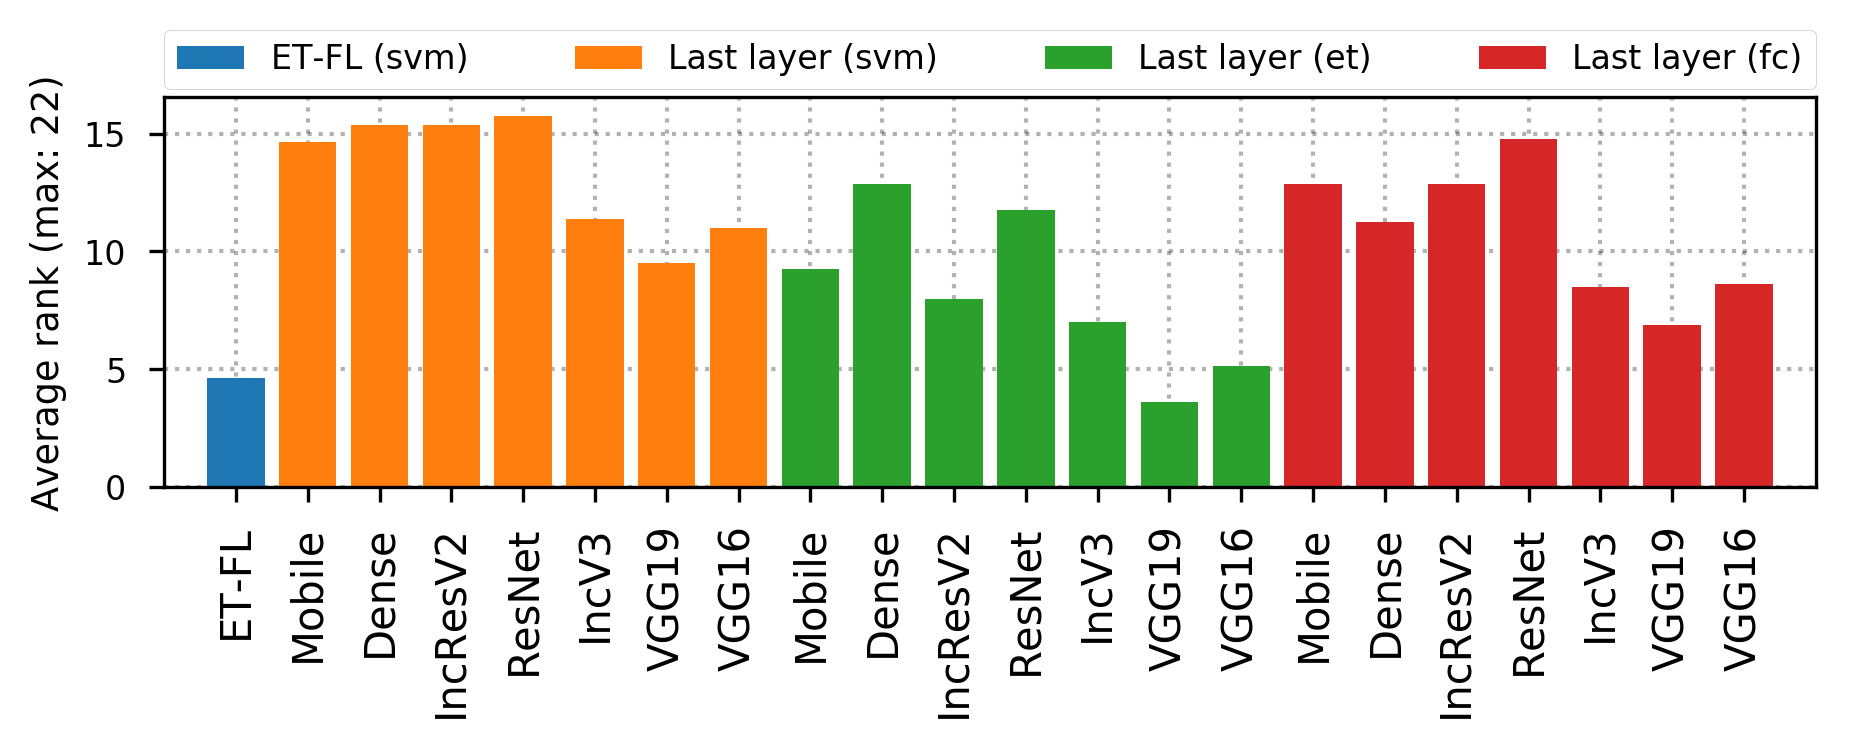
\includegraphics[scale=0.52]{comp/last_baseline_bars.png}
     \caption{Average ranks of the methods for the ``\textit{Last layer features}" experiment. Colors encode the choice of classifier for $\mathcal{C}$ (orange for SVM, green for extremely randomized trees and red for single layer perceptron).}
     \label{fig:comp:avg_ranks_last_layer}
 \end{figure}

Our first strategy follows a common approach in biomedical imaging where off-the-shelf features are extracted at the last layer of a pre-trained network. In our case, we take the features from the last feature maps before the first fully connected layer (the numbers of extracted features per network are given in Supplementary Table 4). For each dataset and network, we then tune and train the three types of classifiers $\mathcal{C}$ (ET, SVM, and FC) with the extracted features, on the union of the training and validation sets, and then we evaluate them on the test set. The resulting average ranks for all classifiers and all datasets are given in Figure \ref{fig:comp:avg_ranks_last_layer}.

We observe that SVM and single layer perceptron are more efficient at classifying from deep features than extremely randomized trees, with a slight advantage to SVM. Mobile, DenseNet, IncResV2 and ResNet yield best performances when combined with SVM or single layer perceptron, while for extremely randomized trees, only DenseNet and ResNet are leading the way. Last layer features from VGG16, VGG19 and IncV3 allow most of the time to beat the baseline but they are clearly not competitive with features from the other networks whatever the classifier. Overall, the best performance is obtained by combining ResNet features with SVM.



%-------------------------------------------------------------------------------------------------------------------
\subsection{Last layer feature subset selection}
\label{ssec:comp:exp_feat_sel}


\begin{figure}
	\center 
    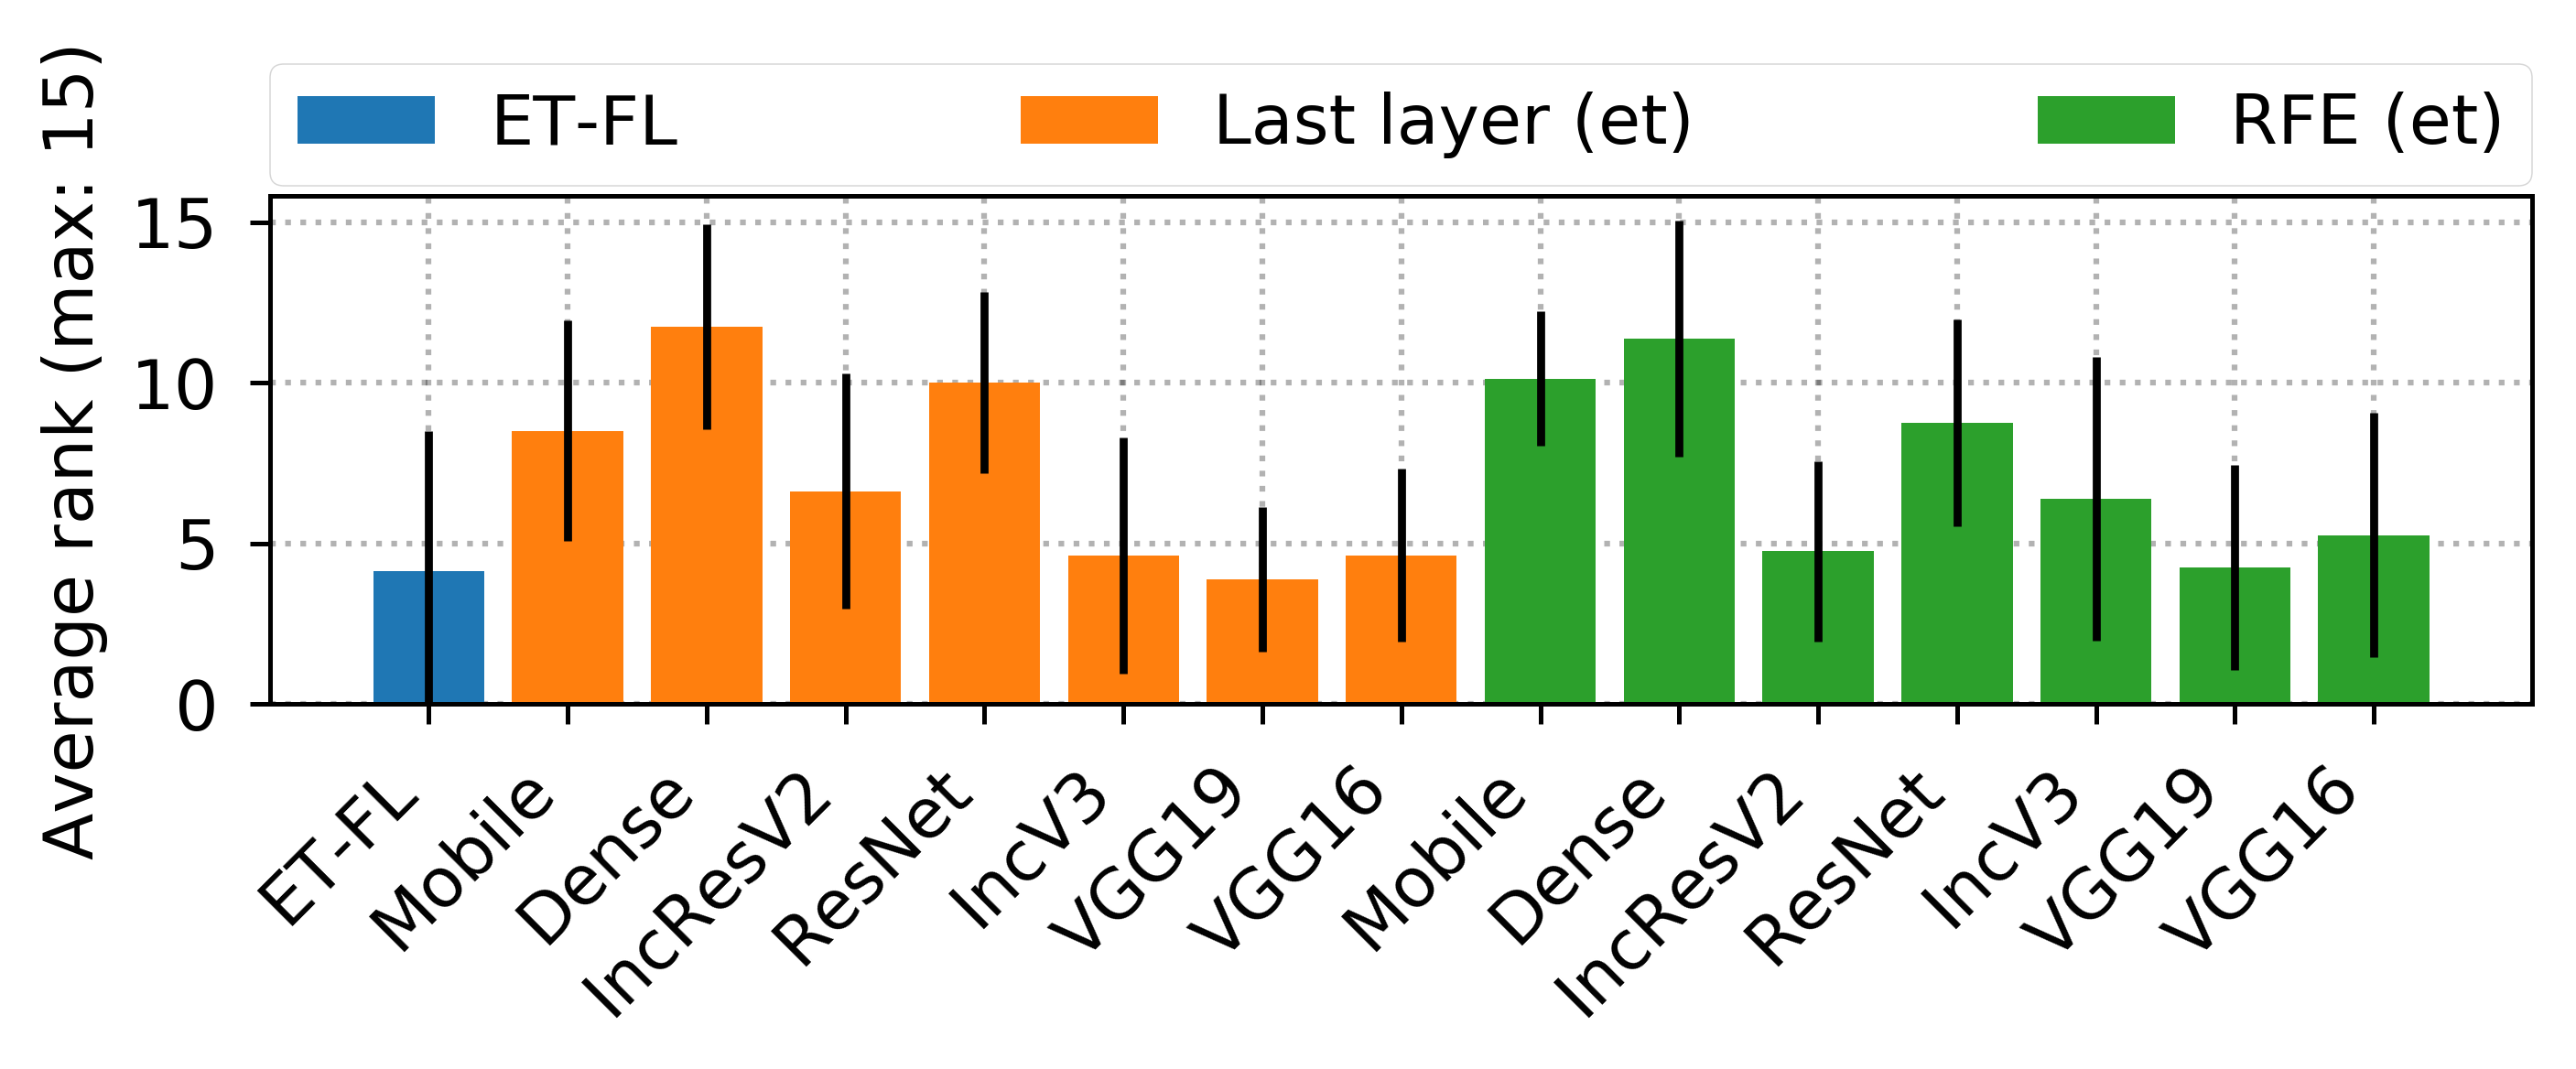
\includegraphics[scale=0.5]{comp/rfe_last_et_bars.png}
    \caption{Average ranks for last layers' features classified with extremely randomized trees before (orange) and after (green) selection with recursive feature elimination.}
    \label{fig:comp:exp_rfe_last_et_cmp}
\end{figure}

%% While carrying out the ``\textit{Last layer features}'' experiment (see Section \ref{ssec:comp:exp_last_layer}), we have analyzed the feature importances produced by extremely randomized trees. We have noticed that few features of the last layer seemed actually important for predicting the outcome.
Our second strategy aims at checking whether all features extracted from the last layer of the network are important for the final classification or if a small subset of them would be sufficient to obtain optimal performance. To answer this question, we use cross-validated recursive feature elimination (RFE) \parencite{guyon2002gene} using importance scores derived from extremely randomized trees to rank the features (where the importance of a given feature is computed by adding up the weighted impurity decreases for all tree nodes where the feature is used, averaged over all trees). This method outputs a sequence $\{(S_t,s_t)|t=1,\ldots,T\}$ (built in reverse), where $S_t$ are nested feature subsets of increasing sizes (with $|S_1|=1$ and $|S_T|=k$) and $s_t$ is the cross-validation performance of an ET model trained on $S_t$. From this sequence, we compute for each dataset:
$$k_{min} = \min_{\{t=1,\ldots,T: s_t\geq \max_{t'} s_{t'}-l_a\}} |S_t|,$$
where $l_a$ is a small performance tolerance (set to $0.005$ in our experiment). $k_{min}$ is thus the minimum number of features needed to reach a performance not smaller than the optimal one by more than $l_a$.

%% Usually, this method consists in taking the number of features that maximizes the cross-validation score. However, in our case, the resulting score curves were flat and noisy (the curves can be found in the Supplementary materials) which led to poor selection of features. Looking at the curves, it was obvious that better subset of features could be taken out of the selected one. We have therefore decided to choose the number of selected features using

%% \begin{equation}
%% \arg \min_{f: s_f \geq m_s - l_a} f
%% \end{equation}

%% where $f$ is a number of features, $m_s$ is the maximum score, $s_f$ is the cross-validation score when $f$ features are selected, $l_a$ is the acceptable loss. The idea is the accept a small loss (\ie we have used $l_a = 0.005$) to reduce even more the number of selected features.

On average across datasets and networks, this method selected 7.5 \% of the features (detailed numbers are given in Supplementary Tables 8 and 9). The models re-trained using the selected features yielded comparable performance when using ET as classifier (see Figure \ref{fig:comp:exp_rfe_last_et_cmp}). Feature selection even improved ET performance on the IncV3, VGG19, and VGG16 networks. Using SVM on the selected features however leads to a performance drop compared to SVM with all features. We believe that this difference is due to the fact that the selection is optimized for ET and it is thus likely to remove features that are useful for linear SVM and not for ET, which are non-linear approximators.

Our experiments show that, among the available features from the last layer, most of them are uninformative or redundant and therefore only few of them are actually needed for the prediction. This conclusion can also be drawn by observing the recursive feature elimination cross-validation curves (see Supplementary Figure 2). For all datasets and networks, the accuracy converges very abruptly to a plateau when the number of selected features increases, which indicates that removing features from the learning set does not impact negatively the predictive power of the models.

It is also interesting to note that the selected features are not the same across datasets. For instance with DenseNet, for a feature to appear in the subset of best features (determined with the importances obtained during the ``\textit{Last layer features}" experiment) for all datasets, we need to consider a subset of size 1477 (\ie 77\% of the features). We observe similar results for the other networks (see Supplementary Table 3). On the other hand, there can be a significant overlap between features selected by RFE for specific pairs of datasets (see Supplementary Table 10). These results suggest that the best features are task-dependent and that there would be no interest in restricting a priori the subset of transferred features, even when focusing on the domain of digital pathology.
 
 
 
\begin{table*}
	\center
    \small
    \begin{tabular}{|l||c|c|c|c|c||c|c|c|}   
      \hline 
      & \multicolumn{8}{c|}{\textbf{Datasets}} \\
      \hline 
      \textbf{Strategy} & \textbf{C} & \textbf{P} & \textbf{G} & \textbf{N} & \textbf{B} & \textbf{M} & \textbf{L} & \textbf{H} \\
      \hline
      Baseline (ET-FL)      & 0.9250 & 0.8268 & 0.9551 & 0.9805	& 0.9345 & 0.7568 & 0.8547 & 0.6960 \\
      Last layer    & 0.9822 & 0.8893 & 0.9938 & \cellcolor{Dandelion}0.9982 & 0.9603 & 0.7996 & 0.9133	& 0.7820 \\
      Feat. select.	& 0.9676	& 0.8861	& 0.9843	& \cellcolor{LimeGreen}0.9994	& 0.9597	& 0.7438	& 0.8941	& 0.7703 \\
      Merg. networks	& \cellcolor{Dandelion}0.9897	& \cellcolor{LimeGreen}0.8984	& 0.9948	& 0.9864	& 0.9549	& \cellcolor{Dandelion}0.8169	& 0.9155	& 0.7928 \\
      Merg. layers	& 0.9808	& 0.8906	& 0.9944	& 0.9964	& 0.9639	& 0.7941	& 0.9268	& 0.7977 \\
      Inner ResNet	& 0.9748	& \cellcolor{Dandelion}0.8959	& 0.9949	& 0.9964	& 0.9664	& 0.8131	& \cellcolor{Dandelion}0.9291	& \cellcolor{Dandelion}0.8113 \\
      Inner DenseNet	& 0.9862	& \cellcolor{LimeGreen}0.8984	& \cellcolor{Dandelion}0.9962	& 0.9917	& 0.9699	& 0.8012	& 0.9268	& 0.7967 \\
      Inner IncResV2	& 0.9873	& 0.8948	& \cellcolor{Dandelion}0.9962	& \cellcolor{Dandelion}0.9982	& \cellcolor{Dandelion}0.9720	& 0.8137	& 0.9234	& 0.7713 \\
%       Inner IncV3		& 0.9836	& 0.8899	& 0.9951	& 0.9964	& 0.9731	& 0.8104	& 0.9201	& 0.7507 \\
       Fine-tuning		& \cellcolor{LimeGreen}0.9926	& 0.8797	& \cellcolor{LimeGreen}0.9977	& 0.9970	& \cellcolor{LimeGreen}0.9873	& \cellcolor{LimeGreen}0.8727	& \cellcolor{LimeGreen}0.9405	& \cellcolor{LimeGreen}0.8641 \\
%%      \hline
%%      \textbf{Best} & 0.9926 & 0.8984 & 0.9977 & 0.9994 & 0.9873 & 0.8727 & 0.9405 & 0.8641 \\
      \hline
      \textbf{Metric} & \multicolumn{5}{c||}{Roc AUC} & \multicolumn{3}{c|}{Accuracy (multi-class)} \\
      \hline
	\end{tabular}
      \caption{Best score for each strategy and each dataset. The best and second best scores are respectively highlighted in green and orange.}
    \label{tab:comp:res_best_scores_per_strategy}
\end{table*}



 %-------------------------------------------------------------------------------------------------------------------
\subsection{Merging features across networks}
\label{ssec:comp:exp_merge_net}


 \begin{figure}
     \center 
     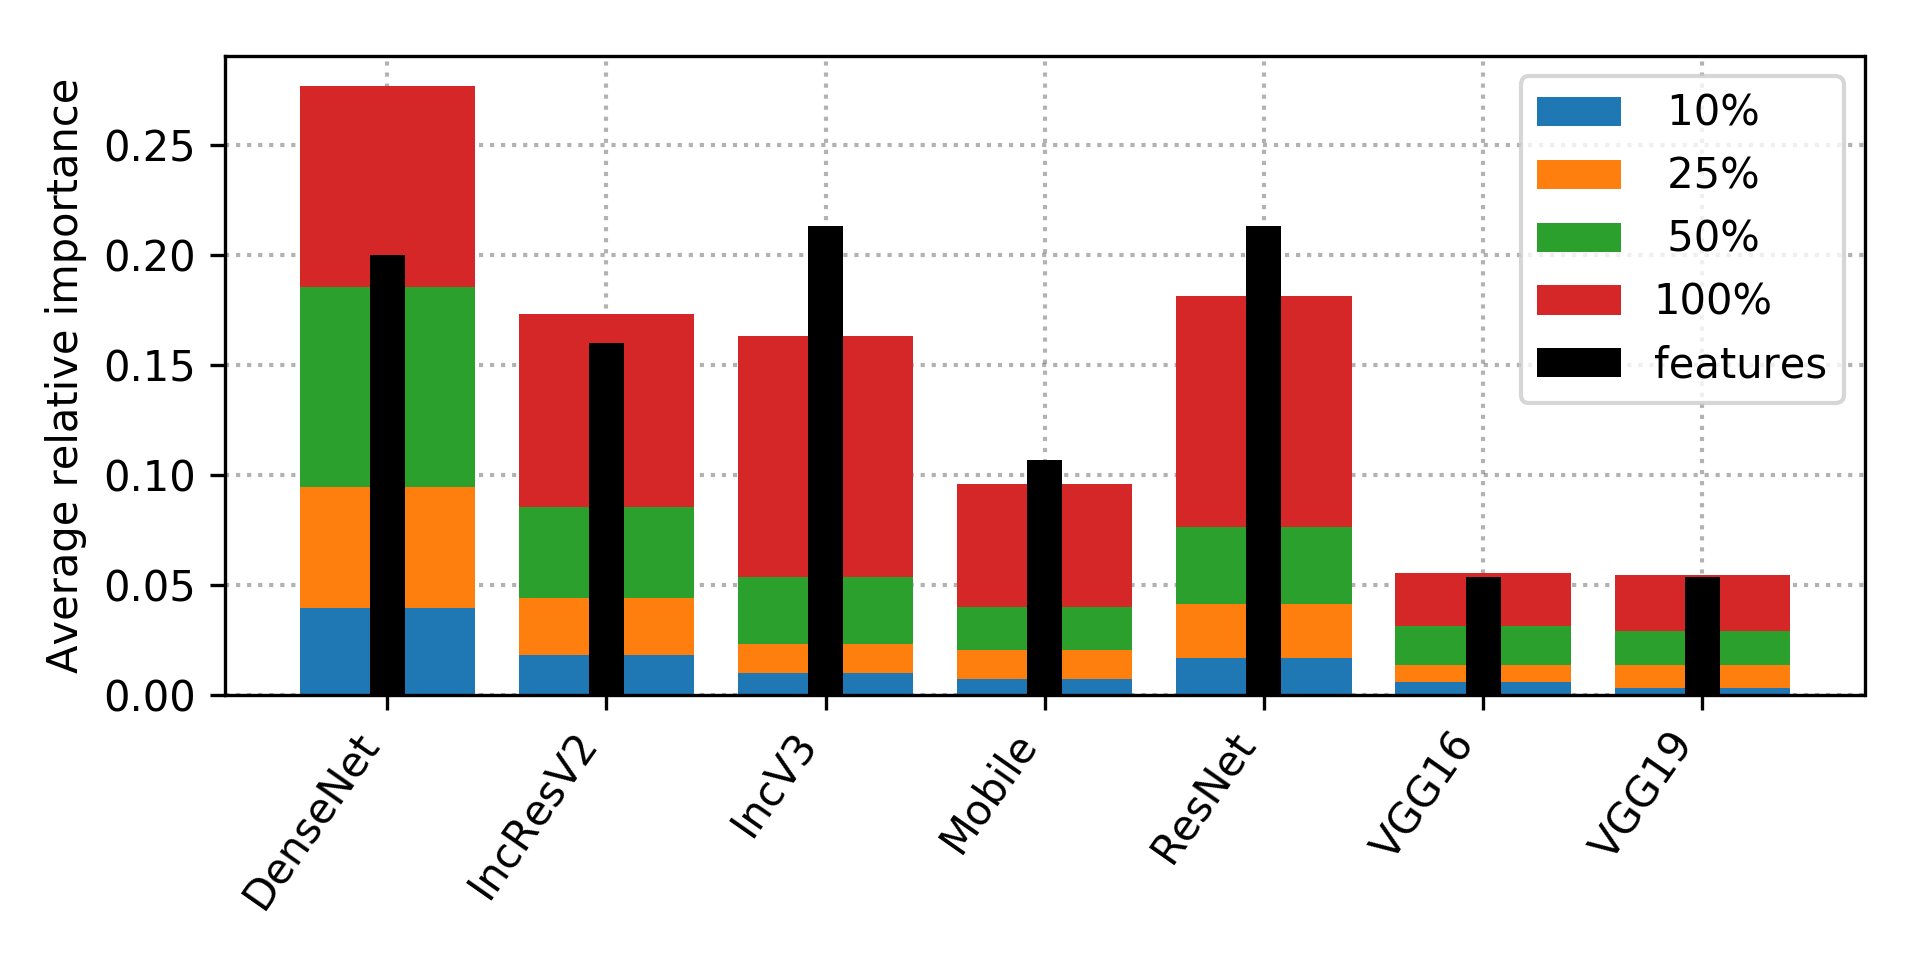
\includegraphics[scale=0.5]{comp/merged_all_merged_perc.png}
     \caption{Average relative importances (across datasets) brought by each studied network when all their last layer features are aggregated. The black bars quantify the proportion of features of each network. The colors indicate the information brought by features of decreasing importances: blue and red features are respectively the most informative and least informative ones. Blue, orange, green and red bars regroup importances of features that respectively and cumulatively bring 10\%, 25\%, 50\% and 100\% of the information for predicting the outcome.}
     \label{fig:comp:models_merged_avg_imp}
 \end{figure}


The third strategy consists in merging features from the last layer of all the studied networks. Aggregating all features results in a feature vector of size $9600.$ We observe in Table \ref{tab:comp:res_best_scores_per_strategy} and Figure \ref{fig:comp:res_avg_ranks_all_methods} that despite the fact that features from all networks are combined, this strategy gives performance results similar to but not better than using the best single network, both with ET and SVM.

Using forest importance ranking procedure described previously, we further analyze the information brought by the last layer of each network (feature importances averaged across datasets are given in Figure \ref{fig:comp:models_merged_avg_imp}). We observe that the features of DenseNet bring more than 25\% of information on average while they only account for 20\% of all the features. Moreover, the proportion of information brought by the most informative features of DenseNet is higher than for any other network. Following DenseNet, the next most informative networks are IncResV2, ResNet, IncV3 and finally the Mobile, VGG16 and VGG19 networks. 
Surprisingly, the importances brought by the VGG networks relatively to the number of features is non-negligible and higher than the one of ResNet and IncV3. This may indicate that features of those networks are redundant with features of DenseNet and IncResV2 while features of VGG16 and VGG19 are not.



%-------------------------------------------------------------------------------------------------------------------
\subsection{Merging features across layers}
\label{ssec:comp:exp_merged_layers}

\begin{figure}
     \center 
     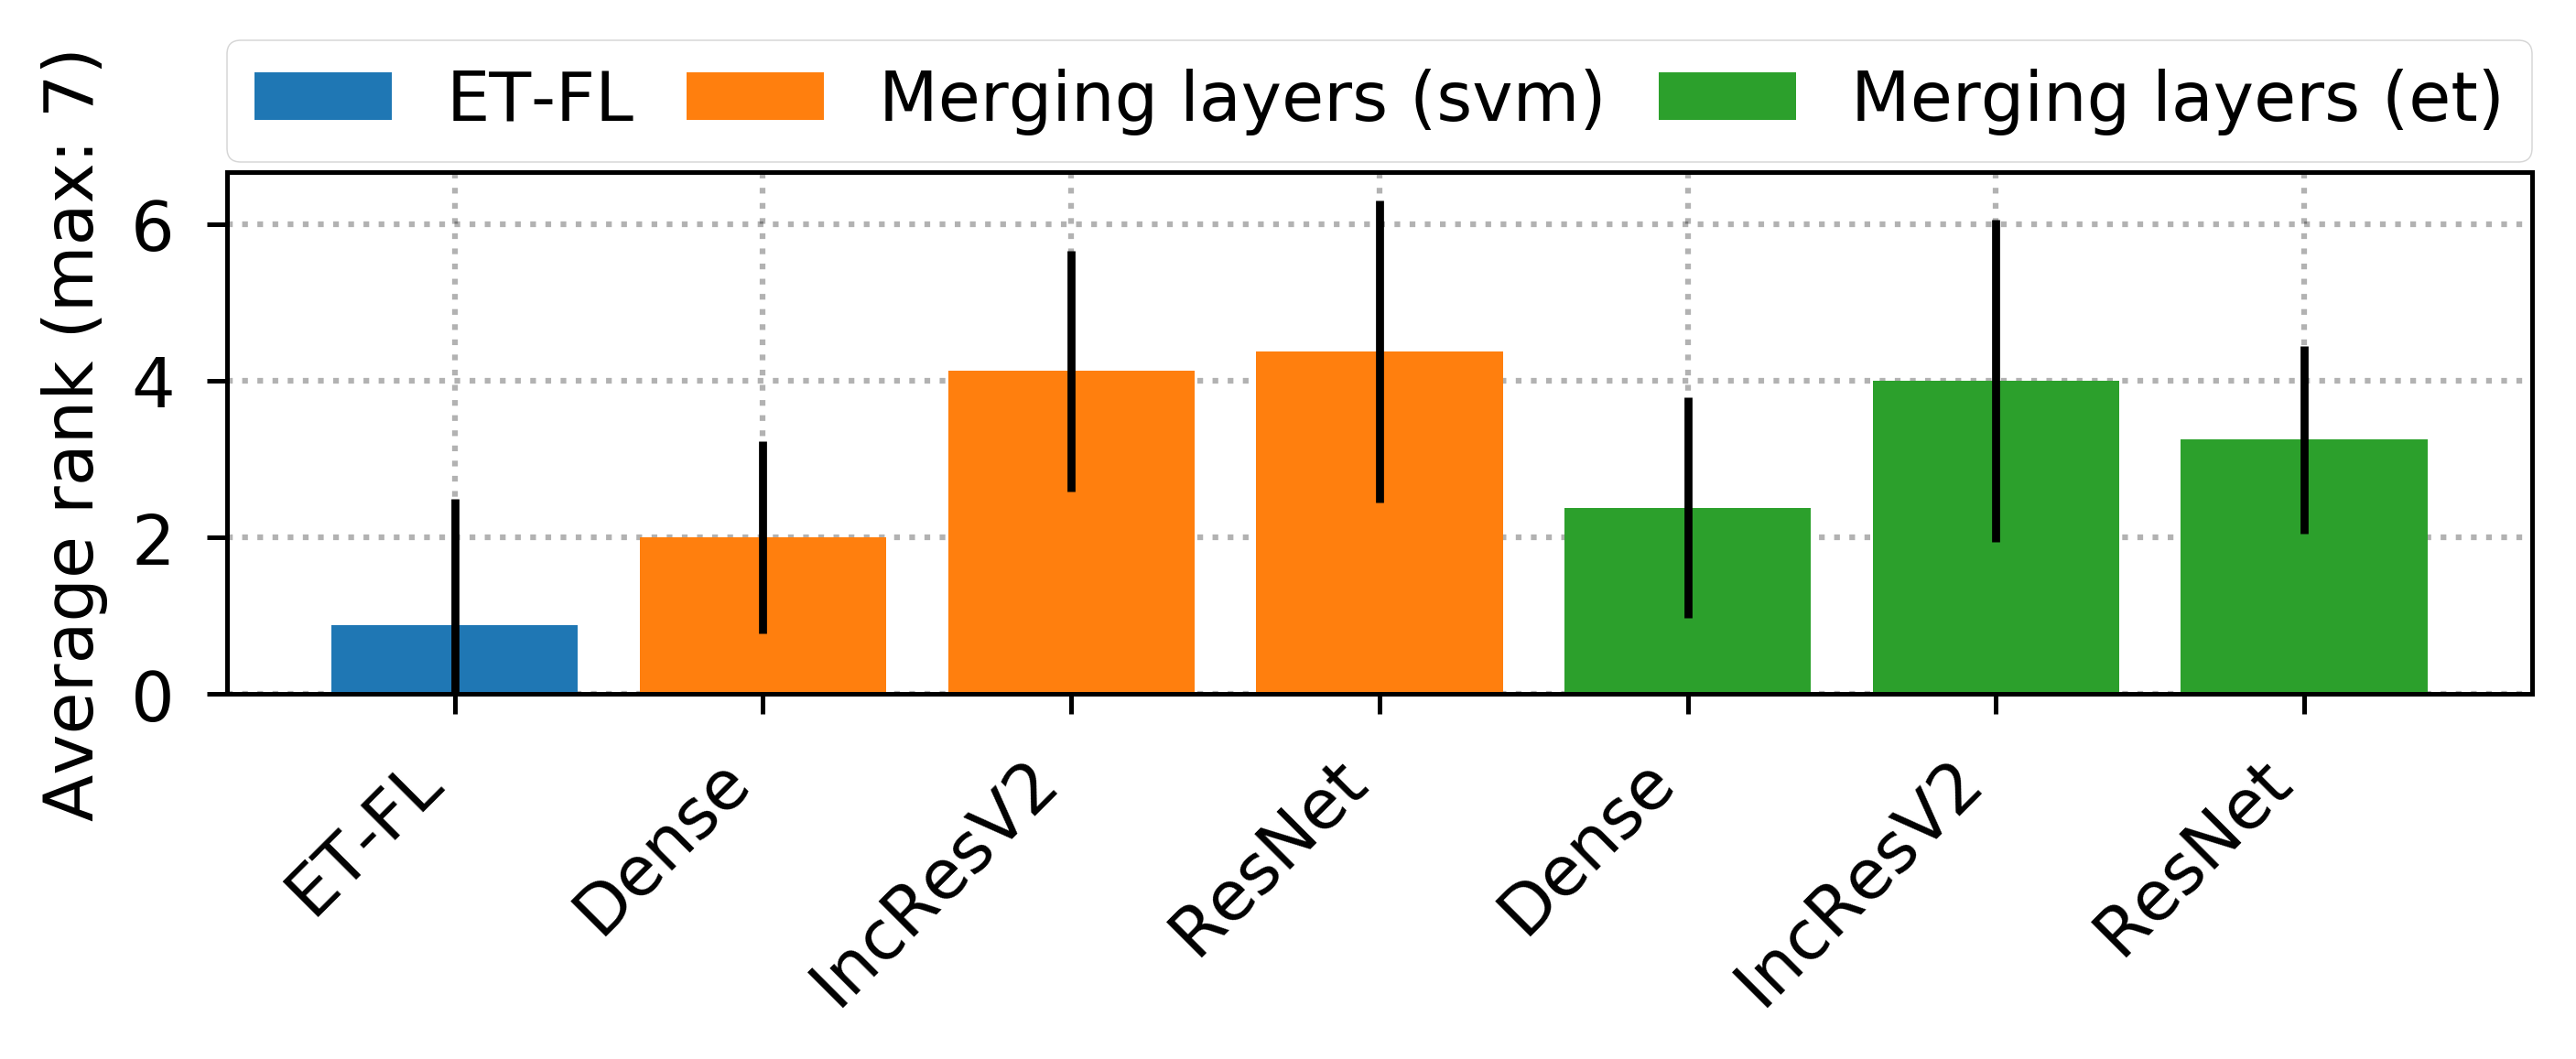
\includegraphics[scale=0.525]{comp/merged_layers_all_bars.png}
     \caption{Average ranks for models learned on merged layers of networks compared to the baseline.}
     \label{fig:comp:res_avg_ranks_merged_layers}
 \end{figure}
 

 
  \begin{figure}
     \center 
     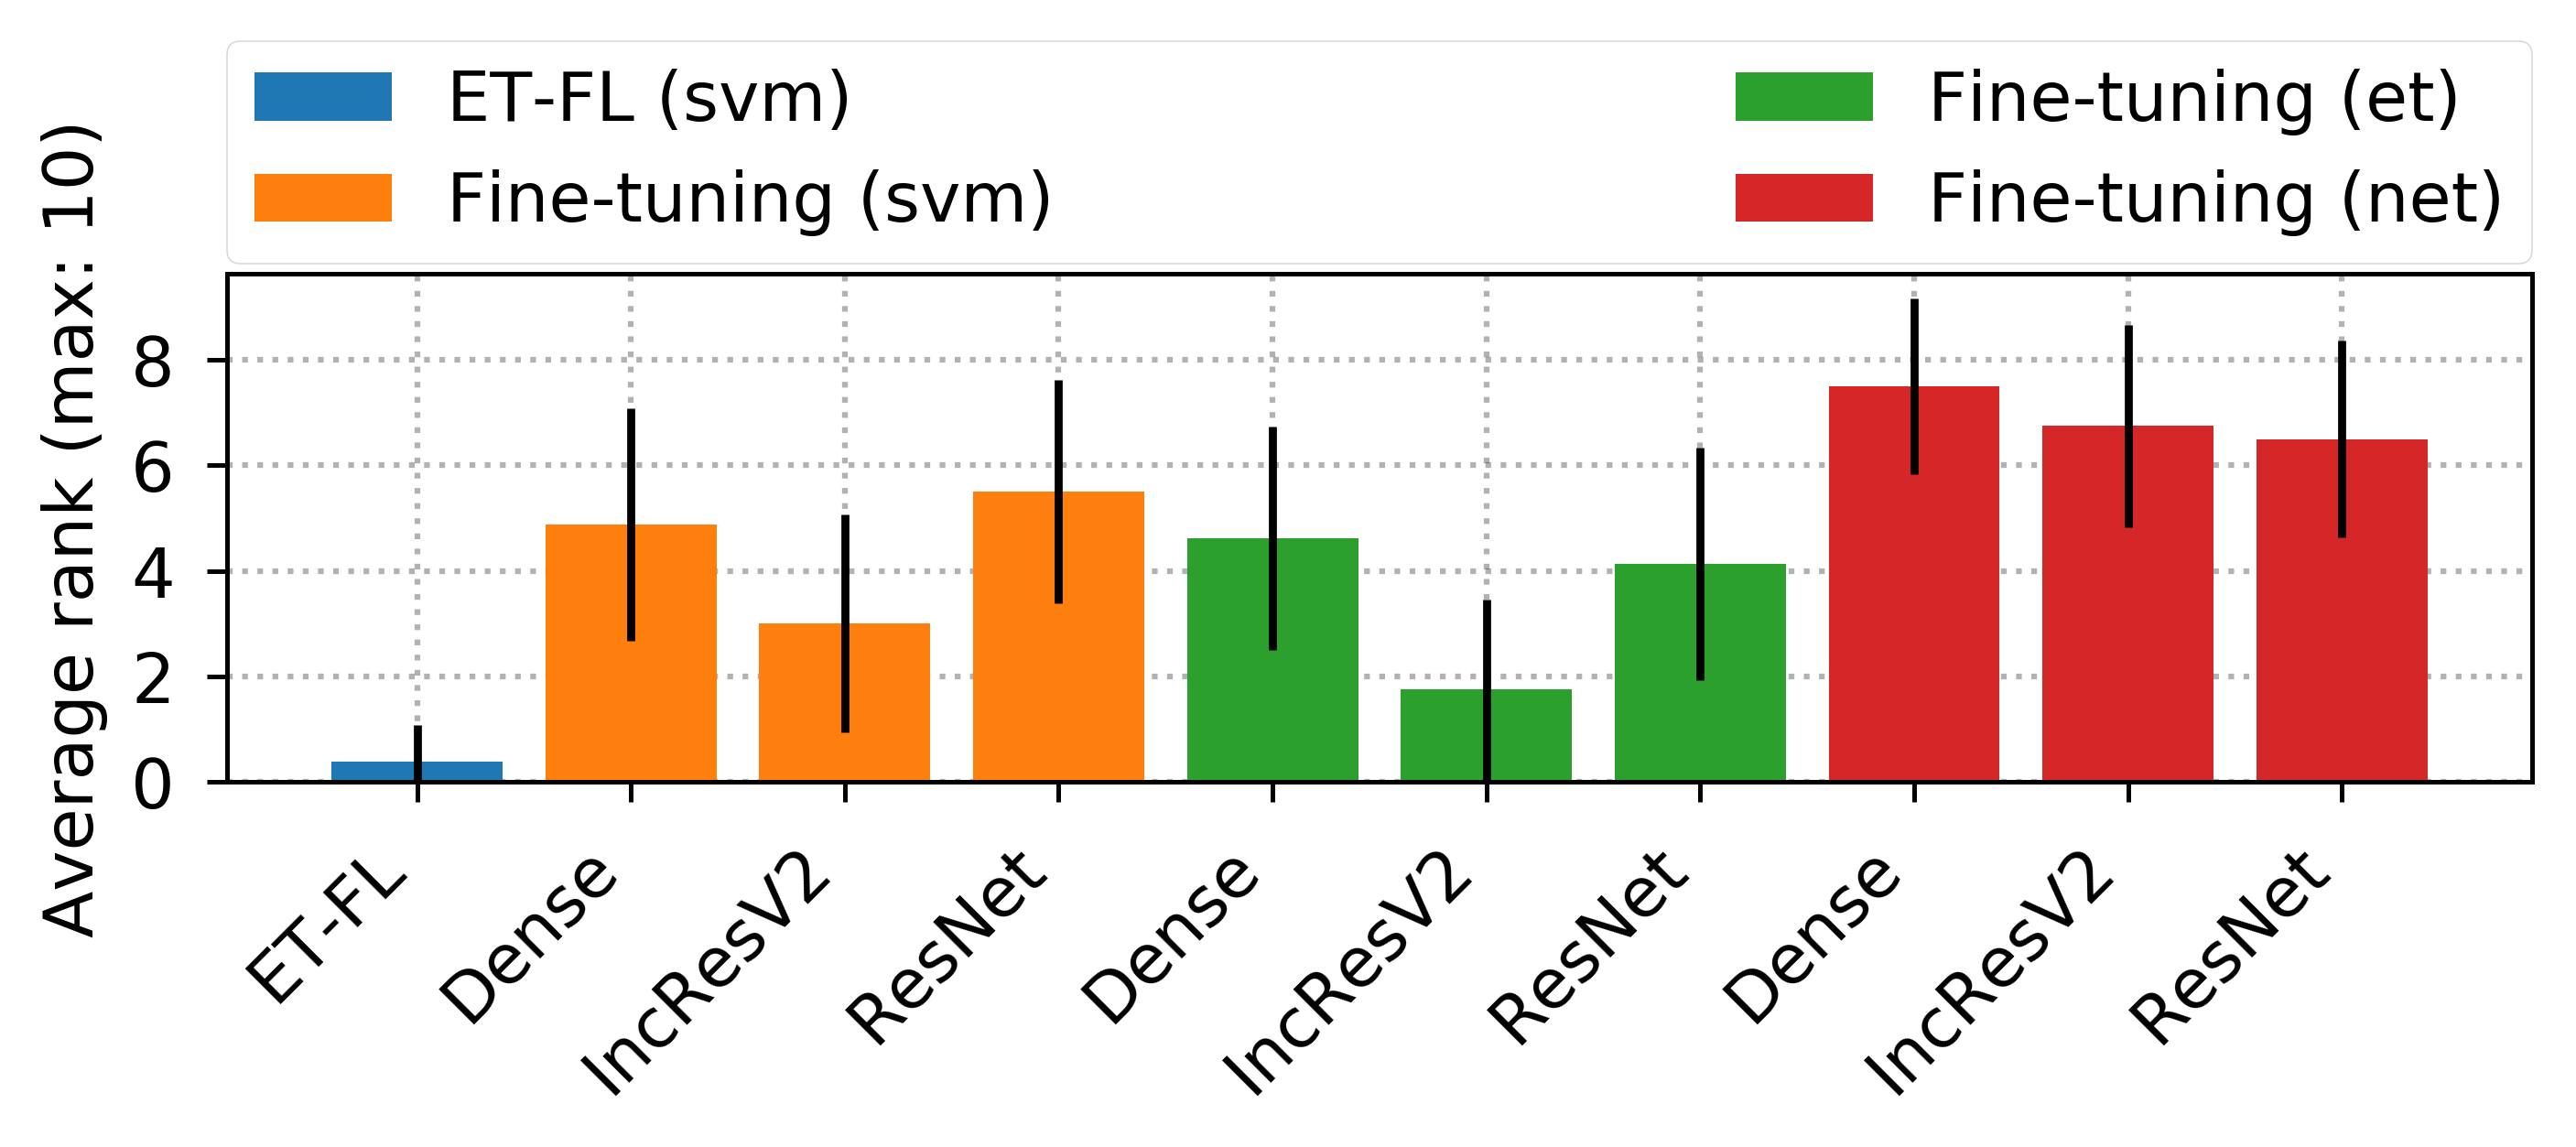
\includegraphics[scale=0.525]{comp/ft_baseline_bars.png}
     \caption{Average ranks for fine-tuned networks compared to the baseline. Evaluation was done either by using SVM (orange) or extremely randomized trees (green) on the fine-tuned features or by predicting the outcome using the fine-tuned fully-connected layer directly (red).}
     \label{fig:comp:res_avg_ranks_ft}
 \end{figure}

This strategy aims at merging features across layers (at several depths) for a given network. Given the results in Section \ref{ssec:comp:exp_last_layer}, we limit our analysis to the IncResV2, ResNet and DenseNet networks. Those three networks have complex structures and many layers which yield plenty of possible cut points for feature extraction. To reduce the number of possibilities, we limit the extraction to bottlenecks of the networks. Details about the layer selection are given in Supplementary Section D. 

The average ranks for each layer of all studied networks are given in Figure \ref{fig:comp:res_avg_ranks_merged_layers}. One first observation is that there is no significant difference between SVM and ET in terms of performance, unlike when we use the last layer only. Surprisingly, DenseNet is not performing well with respect to the other network while it was competitive with using the last layer only. Merging the layers actually leads to a drop of performance with respect to using only the last layer for DenseNet, while it leads to a small improvement for the other two networks (see Section \ref{ssec:comp:exp_comparing}).

As in the previous section, we use feature importances to identify most informative features. Detailed importances plots for each network can be found in Supplementary Figure 1. These plots clearly show that the most informative features are spread over all layers. We also observe that the relative importance of features in the early layers is higher than the ones in deeper layers. One possible reason is that last layers actually have more features than earlier ones and as shown in Section \ref{ssec:comp:exp_feat_sel}, most of those features are either irrelevant or redundant. Therefore, the extremely randomized trees actually discard most of them them during training. 

Merging features from several layers results in large feature vectors for describing the images. Those large vectors make this method less attractive as it results in longer classifier training time. This is especially true for extremely randomized trees. Unlike in the previous strategy however, feature extraction does not increase computation requirements as only one forward pass through the network is needed to extract all the features.



%-------------------------------------------------------------------------------------------------------------------
\subsection{Inner layers features}
\label{ssec:comp:exp_inner_layers}

\begin{figure}
     \center 
     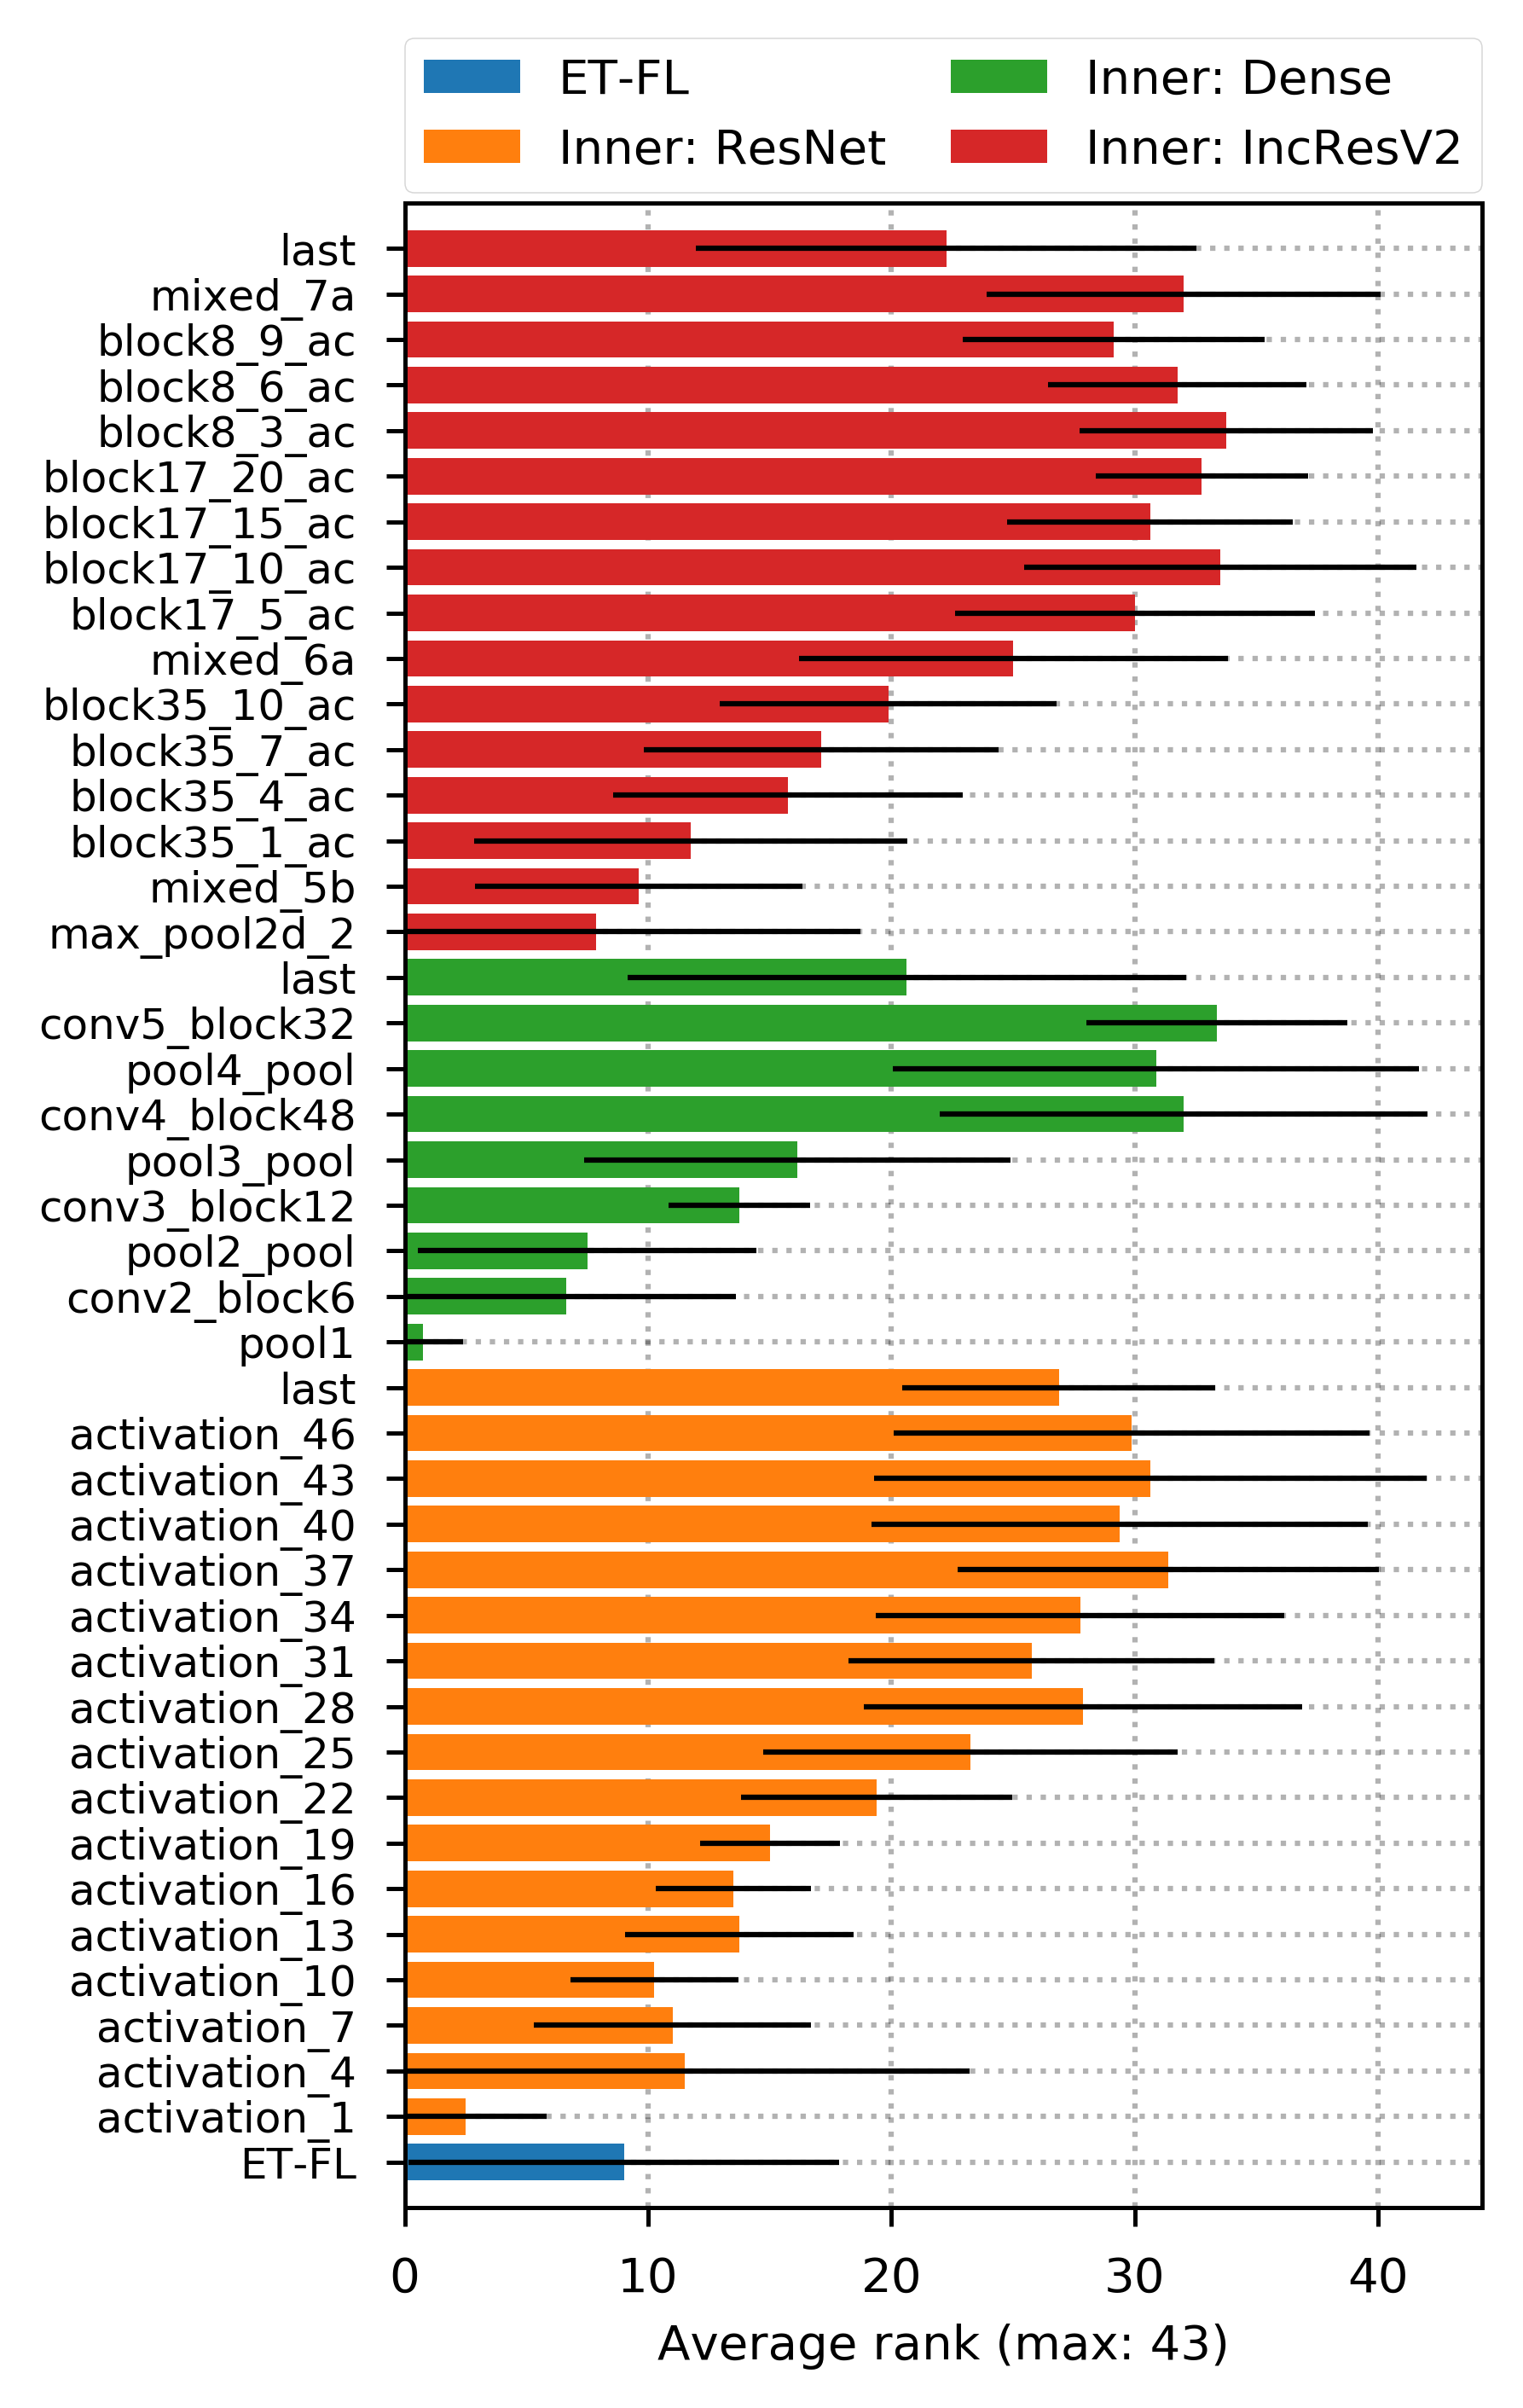
\includegraphics[scale=0.8]{comp/all_per_layer_bars.png}
     \caption{Average ranks for the baseline and the models trained using features from layers inside the networks. For each network, the layers are sorted by decreasing depth (from top to bottom).}
     \label{fig:comp:res_avg_ranks_per_layer}
 \end{figure}
 
For this strategy, we assess features extracted from each layer separately. The motivation is to determine if there is a layer that, taken alone, yields better performance than the others, and in particular, the last one. Using the same cut points as in the previous section to define the layers, we learn as many SVM classifiers as there are layers, each using the features of a single layer.

Average ranks for each inner layer and each network are given in Figure \ref{fig:comp:res_avg_ranks_per_layer}. In all cases, the last layer features are always outperformed by features taken from an inner layer of the network. The optimal layer is however always located rather at the end of the network, while the first layers are clearly never competitive. Unfortunately, we have not found that a specific layer was better for all datasets, so in practice the choice of the layer should be determined by internal cross-validation as we did. Interestingly, the baseline either outperforms the early layers of the networks or yield comparable results which tends to indicate that the features provided by ET-FL are somewhat low-level.

%-------------------------------------------------------------------------------------------------------------------
\subsection{Fine-tuned features}
\label{ssec:comp:exp_fine_tuning}

All previous experiments explored strategies using off-the-shelf features. In this last strategy, we investigate fine-tuning as described in Section \ref{ssec:comp:meth_fine_tuning}. We focus on the same three networks as in the previous sections (ResNet, IncResV2 and DenseNet).

The average ranks for the different fine-tuning methods are given in Figure \ref{fig:comp:res_avg_ranks_ft}. With the three networks, best performances are obtained by making predictions directly from the fine-tuned fully connected layer. SVM and ET trained on the features extracted from the fine-tuned networks are clearly inferior, in particular with IncResV2. Note that, for the other two, last layer features extracted from the fine-tuned network are nevertheless better than last layer features from the original network, when used as inputs to SVM (see Figure \ref{fig:comp:res_avg_ranks_all_methods}). Fine-tuning is thus globally improving the quality of the features for these two networks. Overall, the best performance is obtained with fine-tuned DenseNet.



%-------------------------------------------------------------------------------------------------------------------
%-------------------------------------------------------------------------------------------------------------------
\subsection{Discussion}
\label{ssec:comp:exp_comparing}



To allow comparison of all strategies, the best scores per strategy and dataset are summarized in Table \ref{tab:comp:res_best_scores_per_strategy} and the average ranks of all methods evaluated in the previous experiments are given in Figure \ref{fig:comp:res_avg_ranks_all_methods}.

Concerning the networks, ResNet and DenseNet often yield the best performing models whatever the way they are exploited. They are followed by the IncResV2, Mobile, and IncV3 networks. Performances obtained with the VGG networks are below those of the others.

Concerning the methods, fine-tuning (and predicting with the network) usually outperforms all other methods whatever the network. Especially, this strategy yields significant improvements for the multi-class datasets. For binary datasets, the improvement is often not as impressive, but on three of these datasets, the performances of all methods are already very high (greater than 0.9).

Moreover, for each dataset, there is at least one inner layer that yields the best or second best scores and this best layer is never the last one. This is confirmed by the rank plot that shows that the ranks of the models learned on last layer features are below those using inner layer features. This might be explained by the fact that last layer features are too specific to the source task (natural images).

Merging features across networks and layers yield results similar to using last layer features but they are outperformed by the best inner layers and also by fine-tuning. The inferior performances of these methods could be attributed to the fact that important features are lost among many redundant and uninformative ones and they are thus suffering from overfitting. One way to improve these methods could be to perform feature selection. However, given that these methods are already more computationally demanding, they are definitely less interesting than fine-tuning and selecting the best inner layer. In particular, merging features across networks requires a forward-pass through all the selected networks. Although only one pass is needed when merging the layers, it still yields a large feature vector which makes further training and tuning slower, especially for ET.

Throughout the experiments, we have also gained more insights about the extracted features. By performing feature selection, we have discovered that very few features are actually useful for learning efficient classifiers on our datasets and the best features are task-dependent.




%-------------------------------------------------------------------------------------------------------------------
%-------------------------------------------------------------------------------------------------------------------
\section{Conclusion}

In this work, we have empirically investigated various deep transfer learning strategies for recognition in digital pathology and microscopy. 
We have observed that residual and densely connected networks often yielded best performances across the various experiments and datasets. We have also observed that fine-tuning outperformed features from the last layer of off-the-shelf networks. It also appeared that using one network's inner layer features yielded performances slightly superior to using those of the last layer and inferior to fine-tuning but with the advantage of not having to re-train the network. We hope our thorough study and our results will help practitioners to devise best practices for efficient usage of existing deep networks. 

In the future, we want to study further deep transfer learning (e.g. combining inner layers and fine-tuning strategies). We also aim at collecting and merging larger annotated biomedical datasets to train networks using a large-scale source dataset closer to our target tasks.  We also plan to integrate these strategies into the Cytomine \parencite{maree2016collaborative} web application to ease their application on novel datasets.


% \section*{Acknowledgments}
% R. Mar\'ee is supported by grant ``IDEES" (Wallonia / ERDF). Computing resources have been provided by Prof. Marc Van Droogenbroeck and by the GIGA Institute. This work is partially supported by the Belspo project INSIGHT (BRAIN-be). We thank our collaborators for providing images and  annotations (see Supplementary Section H).

\begin{figure}
  \center 
  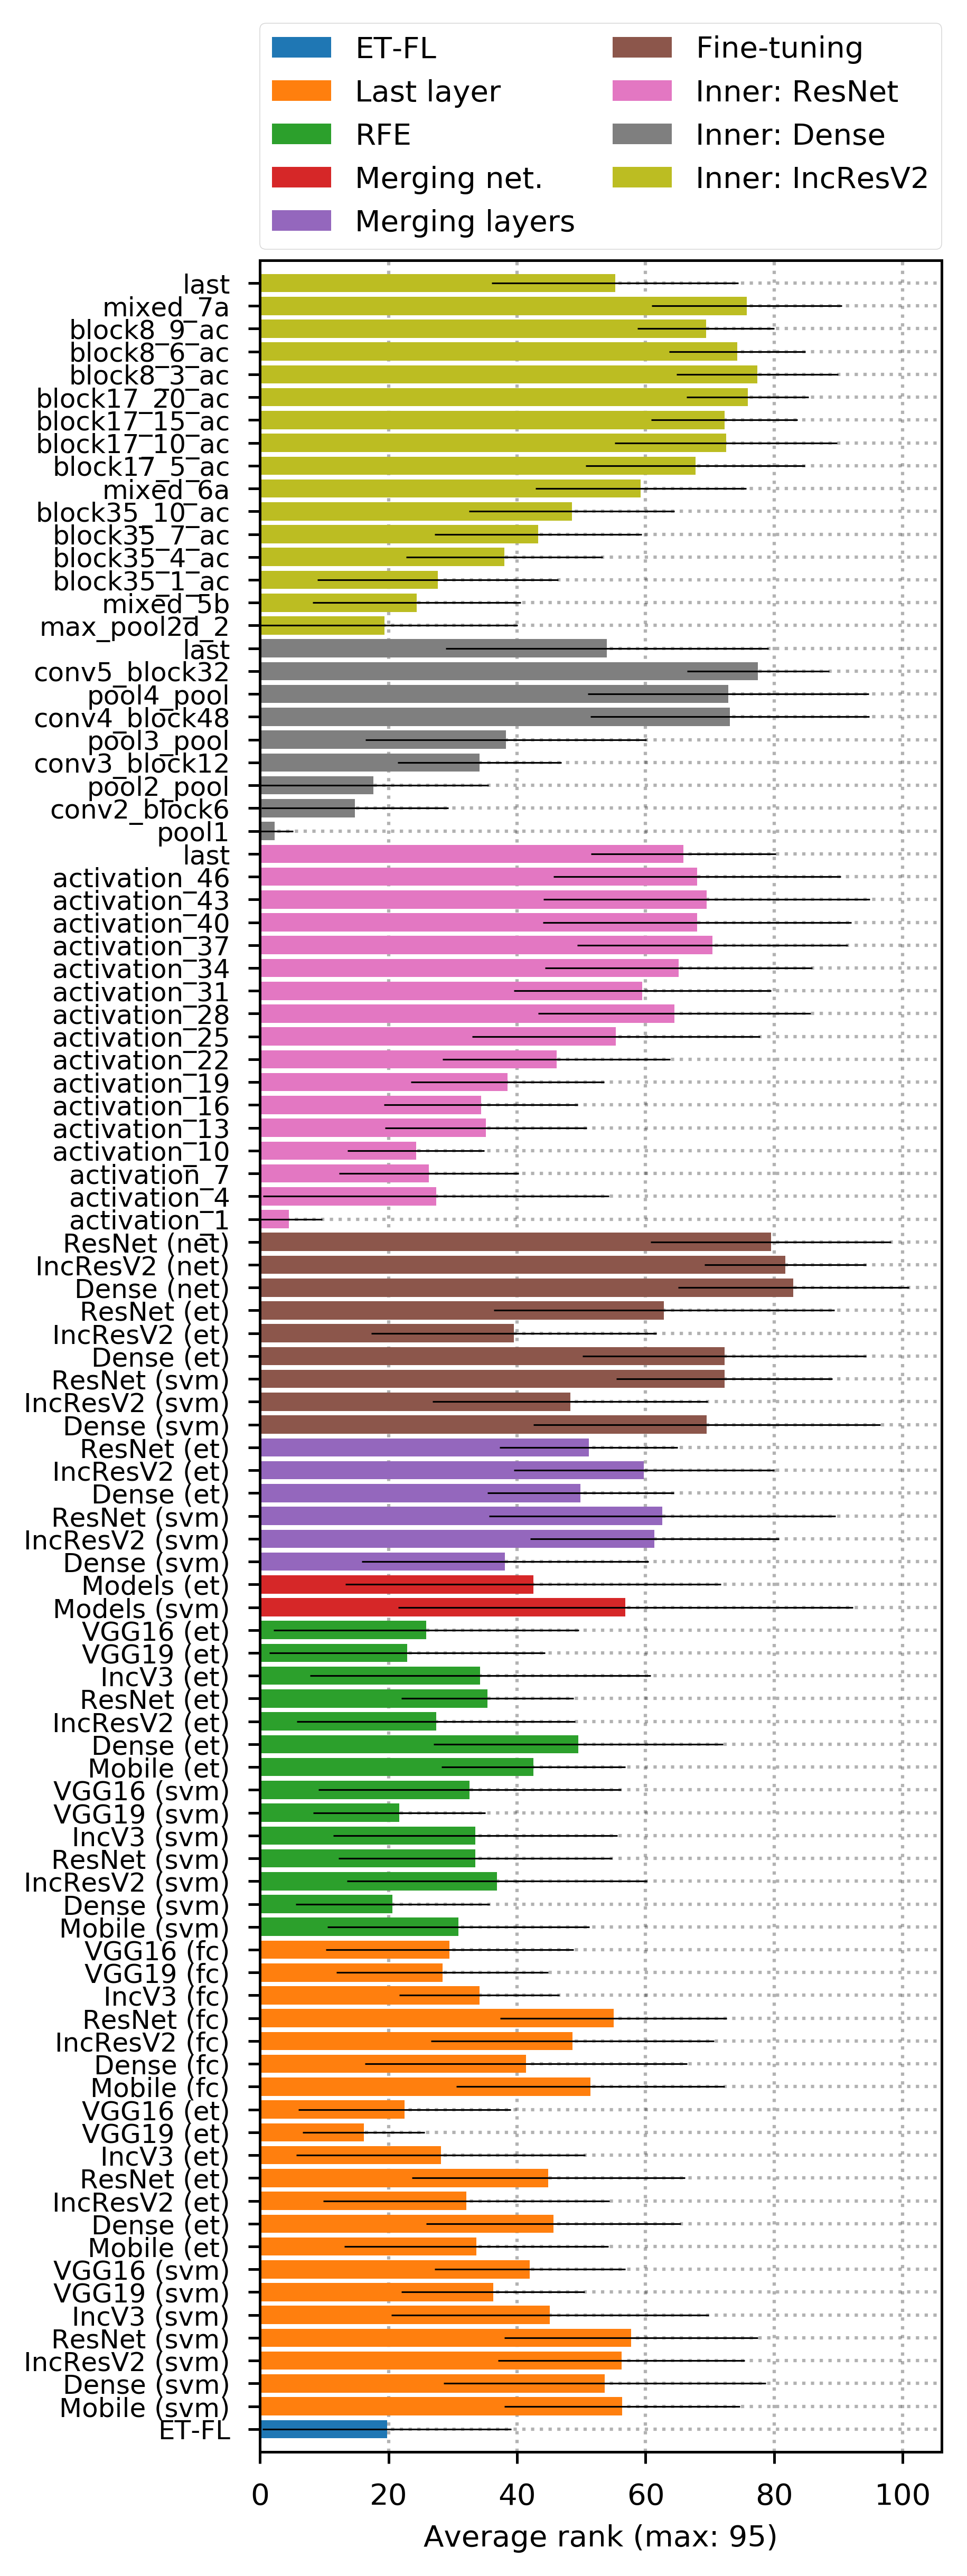
\includegraphics[scale=0.85]{comp/all_exp_bars.png}
  \caption{Average ranks for all the evaluated methods.}
  \label{fig:comp:res_avg_ranks_all_methods}
\end{figure}